\section{Mapa i orientacja przestrzenna}
    Jednym z założeń projektu było napisanie dedykowanej aplikacji graficznej do sterowania pojazdem oraz prezentacji mapy.
    Na rysunku \ref{fig:app} przedstawiono interfejs tego programu, który składa z trzech części:
    \begin{figure}[!ht]
        \centering
        \includegraphics[width = 0.7\textwidth]{PathFinding/App.png}
        \caption{Interfejs aplikacji}
        \label{fig:app}
    \end{figure}
    \begin{enumerate}
        \item Mapa -- reprezentująca zbadany obszar oraz obecną pozycję pojazdu.
        \item Informacje -- w prawym górnym rogu wyświetlane są dodatkowe komunikaty, takie jak aktualne współrzędne samochodu, czy myszy.
        \item Ślizgacze -- w prawym dolnym rogu znajdują się dwa ślizgacze, górny umożliwia ustawienie kąta skrętu kół, a dolny pozwala na regulację prędkości pojazdu.
    \end{enumerate}

    \subsection{Wyszukiwanie ścieżek}
        W zamyśle program ma za zadanie jedynie wyświetlać mapę zbudowaną przez samochód, natomiast wszelkie obliczenia powinny zostać wykonane przez mikrokontroler.
        Jednak ze względu na dosyć skomplikowane przetwarzanie uzyskanych danych w celach testowych, to aplikacja posiada implementację przedstawionych algorytmów.

        Aby wytyczyć trasę, po której będzie poruszał się pojazd na narysowanej przestrzeni, należy wskazać punkt docelowy.
        W chwili kliknięcia rozpoczyna się złożony proces, który można podzielić na kilka podpunktów:
        \begin{enumerate}
            \item wyszukanie połączenia między dwoma miejscami,
            \item zamiana listy punktów na instrukcje,
            \item wygładzenie zakrętów.
        \end{enumerate}
        Wszystkie te elementy muszą działać niezawodnie, ponieważ błąd na którymkolwiek etapie, może mieć katastrofalne skutki.

        \subsubsection{Algorytm odnajdowania drogi}
        \label{subsec:algorytm_odnajdowania_ścieżek}
            Wyznaczanie optymalnej ścieżki, od wielu lat jest powszechnym problemem w informatyce i~robotyce.
            Istnieje mnóstwo artykułów, skupiających się na tej tematyce, a także ogrom gotowych rozwiązań.
            Do najpopularniejszych należą:
            \begin{itemize}
                \item algorytm A* (A star),
                \item algorytm Dijkstry,
                \item algorytm Bellmana-Forda.
            \end{itemize}

            Poniżej zaprezentowano wyniki pracy \citetitle{AnalizaAlgorytmówŚcieżek} \cite{AnalizaAlgorytmówŚcieżek}.
            \begin{figure}[!ht]
                \centering
                \includegraphics[width=0.65\textwidth]{PathFinding/Wykres_sredni_czas_algorytmu_pathfinding.png}
                \caption{Wykres porównania średniego czasu wykonania algorytmów}
                Źródło:\cite{AnalizaAlgorytmówŚcieżek} \citetitle{AnalizaAlgorytmówŚcieżek}
                \label{fig:PathFindingTime}
            \end{figure}
            \begin{figure}[!ht]
                \centering
                \includegraphics[width=0.65\textwidth]{PathFinding/Wykres_sredni_koszt_algorytmu_pathfinding.png}
                \caption{Wykres porównania średniego kosztu znalezionych ścieżek}
                Źródło:\cite{AnalizaAlgorytmówŚcieżek} \citetitle{AnalizaAlgorytmówŚcieżek}
                \label{fig:PathFindingCost}
            \end{figure}

\newpage
            Na podstawie przedstawionego artykułu można wywnioskować, że najlepsze rozwiązanie to algorytm Dijkstry.
            Jego złożoność stanowi dodatkowy czynnik potwierdzający powyższe stwierdzenie.
            Jest on stosunkowo prosty w implementacji, a co więcej posiada niski koszt obliczeniowy.
            Dzięki temu wydaje się trafnym wyborem dla zastosowań w układach embedded.

    \subsection{Wygładzanie ścieżek}
    \label{subsec:wygładzanie_ścieżek}
        Rysunek \ref{fig:pathfinding_dikstra} prezentuje przykładową drogę, wyznaczoną przez algorytm Dijkstry,
        który zwraca najkrótsze połączenie między dwoma punkami, będące prostą.
        Jednak ze względu na ograniczenia konstrukcyjne wyrysowana trasa jest niemożliwa do pokonania przez robota.

        \begin{figure}[!ht]
            \centering
            \includegraphics[width = 0.7\textwidth, trim = {120px, 30px, 20px, 300px}, clip]{PathFinding/pathfinding_dikstra.png}
            \caption{Przykładowa ścieżka wyznaczona przez algorytm Dijkstry}
            \label{fig:pathfinding_dikstra}
        \end{figure}

        Zbudowany pojazd posiada tylko jedną oś skrętną, więc nie jest w stanie obrócić się w miejscu.
        Koniecznym jest zastosowanie algorytmu wygładzania.
        W artykule \citetitle{Simple_PathSmoothing} \cite{Simple_PathSmoothing} przedstawiona jest najprostsza możliwa metoda zaokrąglania krawędzi.
        Ów algorytm zakłada zapisywanie mapy w postaci listy punktów o niecałkowitych współrzędnych.
        Dzięki temu możliwe jest przesunięcie środka pojedynczej kratki w kierunku łuku skrętu.

        \begin{figure}[!ht]
            \centering
            \includegraphics[width = 0.5\textwidth]{PathFinding/simple_pathSmooth.jpeg}
            \caption{Przykład wygładzania ścieżki na podstawie artykułu}
            \citetitle{Simple_PathSmoothing} \cite{Simple_PathSmoothing}
            \label{fig:simple_pathSmooth}
        \end{figure}

        Opisane rozwiązanie cechuje się niewielkim skomplikowaniem, jednak
        brak możliwości kontroli procesu, a także pocięcie drogi na pojedyncze punkty, między którymi pojazd będzie zatrzymywał się i ponownie ruszał, stanowią olbrzymi minus.
        Dodatkowo pojawia się problem przechowywania mapy w pamięci (sytuacja ta została dokładniej omówiona w rozdziale \ref{subsec:przechowywanie_mapy}).
        W związku z powyższym autor zdecydował się na użycie bardziej skomplikowanego algorytmu.

        Alternatywne metody wygładzenia ścieżek zostały ujęte w dokumentach: \citetitle{Compare_PathSmoothing} \cite{Compare_PathSmoothing} oraz \citetitle{Compare_PathSmoothing2} \cite{Compare_PathSmoothing2}.
        Obie prace przybliżają i~porównują różne sposoby dostosowywania trasy do umiejętności robota.
        Na rysunku \ref{fig:smoothingPath_res} przedstawiono ich wyniki:
        \begin{figure}[!ht]
            \centering
            \begin{minipage}{0.49\textwidth}
                \centering
                \includegraphics[width = \textwidth]{PathFinding/smoothingPath.png}
                Źródło: \cite{Compare_PathSmoothing} \citetitle{Compare_PathSmoothing}
            \end{minipage}
            \begin{minipage}{0.49\textwidth}
                \centering
                \includegraphics[width = \textwidth]{PathFinding/smoothingPath2.png}
                Źródło: \cite{Compare_PathSmoothing2} \citetitle{Compare_PathSmoothing2}
                \vspace{0.5cm}
            \end{minipage}
            \caption{Przedstawienie tras wygładzonych przez różne algorytmy}
            \label{fig:smoothingPath_res}
        \end{figure}

\newpage
        Ostatecznie spośród wszystkich wymienionych w artykułach metod został wybrany algorytm krzywych Dublina, ze względu na łatwą implementację oraz możliwość dostosowywania promienia skrętu.

\newpage
        \subsubsection{Opis algorytmu krzywych Dublina}
            Mechanizm wygładzania ścieżek za pomocą krzywych Dublina jest przeznaczony dla pojazdów o ograniczonej sterowności, przykładowo dla samochodów z tylko jedną osią skrętną.
            \begin{figure}[!ht]
                \centering
                \includegraphics[width = 0.375\textwidth]{PathFinding/dublinCurves.png}
                \caption{Schemat trasy z okręgami o minimalnych promieniach}
                \label{fig:dublinCurves}
                Źródło: \cite{Compare_PathSmoothing} \citetitle{Compare_PathSmoothing}
            \end{figure}

        \begin{wrapfigure}[3]{R}{0.33\textwidth}
            \centering
            \vspace{-1cm}
            \begin{tikzpicture}
                \draw
                    (0,  0.0) node[draw, circle, minimum width = 0.5cm, align=center](A){1}
                    (0, -1.5) node[draw, circle, minimum width = 0.5cm, align=center](B){2}
                    (0, -3.0) node[draw, circle, minimum width = 0.5cm, align=center](C){3}
                    (0, -4.5) node[draw, circle, minimum width = 0.5cm, align=center](D){4}
                    (0, -6.0) node[draw, circle, minimum width = 0.5cm, align=center](E){5}
                    (0, -7.5) node[draw, circle, minimum width = 0.5cm, align=center](F){6}
                ;
                \draw[-Stealth] (A) -- (B);
                \draw[-Stealth] (B) -- (C);
                \draw[-Stealth] (C) -- (D);
                \draw[-Stealth] (D) -- (E);
                \draw[-Stealth] (E) -- (F);
                \draw[-Stealth] (F) to[bend right] (B);

            \end{tikzpicture}
            \caption{Implementacja algorytmu krzywych Dublina zastosowana w projekcie}
        \end{wrapfigure}

        Poniżej przedstawiono implementację algorytmu krzywych Dublina zastosowanego w projekcie.
        Opisana wersja jest nieoptymalną modyfikacją oryginału.

        \vspace{0.25cm}
        \begin{minipage}[l]{0.6\textwidth}
            \begin{enumerate}
                \item Zamiana punktów ścieżki na listę prostych o współrzędnych początkowych i końcowych.
                \item Ustalenie miejsca przecięcia się dwóch kolejnych linii.
                \item Wyznaczenie dwusiecznej kąta, tworzonego przez obie proste w punkcie przecięcia.
                \item Określenie kierunku, w którym samochód będzie poruszał się po zakręcie.
                \item Znalezienie na dwusiecznej środka okręgu, znajdującego się w przeciwnym kierunku do ruchu pojazdu.
                \item Obliczenie punktów styczności okręgu i obu prostych, które stanowią początek i koniec łuku.
            \end{enumerate}
        \end{minipage}
        \vspace{0.25cm}

        Pierwotne założenia mówią, że nie należy łączyć dwóch prostych łukiem, a zawsze o ile jest to możliwe ścieżka powinna zaczynać się i kończyć półokręgiem.
        Jednak w tym projekcie dużo łatwiej jest wyznaczyć łuk wiążący dwie proste, niż trzymać się optymalnej wersji algorytmu.
        Na rysunku \ref{fig:path_dublin} zaprezentowano rezultat wygładzania trasy.

        \begin{figure}[!ht]
            \centering
            \includegraphics[width = 0.7\textwidth]{PathFinding/path_dublinCurve.png}
            \caption{Wyznaczona trasa z wygładzeniem}
            \label{fig:path_dublin}
        \end{figure}



    \subsection{Przechowywanie mapy}
    \label{subsec:przechowywanie_mapy}
        Przechowywanie mapy jest niezwykle złożonym zagadnieniem.
        W zależności od zastosowania oraz platformy, na której pracujemy, mogą istnieć różne sposoby jej przedstawienia.
        Zapisana na komputerze o teoretycznie nieograniczonej dostępnej pamięci, może być bardzo dokładna.
        Natomiast ten sam obraz analizowany przez mikrokontroler o niewielkich zasobach, musi zawierać uproszczenia.

        \subsubsection{Mapa jako tablica ścian}
            W wielu projektach mapa przechowywana jest w postaci dwuwymiarowej tablicy, w której poszczególne komórki odpowiadają określonym polom w labiryncie.
            Każda z nich zawiera informacje, w jakim kierunku można się poruszać.
            Przykład takiej budowy przedstawia artykuł \citetitle{maze_storage}\cite{maze_storage}.
            Na rysunku \ref{fig:mazeCellStorage} zilustrowano proponowane rozwiązanie.

            \begin{figure}[!ht]
                \centering
                \includegraphics[width = 0.7\textwidth]{mazeCellStorage.jpeg}
                \caption{Przechowywanie komórek labiryntu z informacją o możliwości ruchu}
                Źródło: \citetitle{maze_storage}\cite{maze_storage}
                \label{fig:mazeCellStorage}
            \end{figure}

            Metoda ta jest bardzo skuteczna, kiedy znane są dokładne wymiary każdej części badanego obszaru,
            jednak przechowywanie mapy otwartej przestrzeni w podany sposób jest nieefektywne.
            Przykładowo, jeśli z kwadratu $A$ (patrz rys. \ref{fig:dim_issue}), nie da się jechać prosto to może oznaczać zarówno, że w miejscu połączenia z komórką $B$ jest ściana, jak i to, że pole $B$ jest całkowicie nieprzejezdne.
            W labiryncie, gdzie znaczenie mają krawędzie, prezentowane rozwiązanie jest optymalne.
            Jednak jeśli nie jesteśmy w stanie powiedzieć, czy wykrywamy cienką ściankę, czy też dużą przeszkodę, wtedy tracimy jednoznaczność.

            \begin{figure}[!ht]
                \centering
                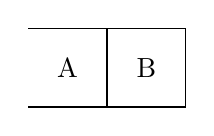
\begin{tikzpicture}
                    \draw
                        (0, 0) -- (1, 0) -- (1, 1) -- (0, 1)
                        (0.5, 0.5) node{A}
                        (1, 0) rectangle (2, 1)
                        (1.5, 0.5) node[]{B}
                    ;
                \end{tikzpicture}
                \caption{Przykład niejednoznaczności wymiarów}
                \label{fig:dim_issue}
            \end{figure}

            Kolejną wadą takiej organizacji danych jest rozmiar pojedynczej komórki oraz czas potrzebny na przeanalizowanie wszystkich dostępnych opcji.
            Każdy kwadrat składa się z 4 bitów,
            co więcej łącząc poszczególne kratki ze sobą, okazuje się, że niektóre bity są nadmiarowe.
            Rozważmy sytuację: jeśli z punktu $A$ (rysunek \ref{fig:bit_issue}) nie możemy jechać do góry, to też, z punktu $C$ nie będzie możliwe przemieszczenie się w dół.
            Informacja dotycząca lokalizacji przeszkód musi zostać zapisana dla każdej komórki osobno.
            \begin{figure}[!ht]
                \centering
                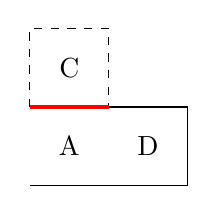
\begin{tikzpicture}
                    \draw
                        (0, 0) -- (1, 0)
                        (1, 0) -- (2, 0) -- (2, 1) -- (1, 1)

                        (0.5, 0.5) node{A}
                        (0.5, 1.5) node{C}
                        (1.5, 0.5) node{D}
                    ;
                    \draw[dashed]
                        (0, 1) rectangle (1, 2)
                    ;
                    \draw[ultra thick, red]
                        (0, 1) -- (1, 1)
                    ;
                \end{tikzpicture}
                \caption{Przykład nadmiarowych informacji}
                \label{fig:bit_issue}
            \end{figure}\\
            Analogiczny problem występuje kiedy trasa jest przejezdna (połączenie między~$A$~i~$D$).

            Podsumowując, powyższa metoda przechowywania mapy jest użyteczna jedynie w przypadku labiryntów o jasno określonych zasadach.
            To rozwiązanie nie sprawdzi się do reprezentacji otwartej przestrzeni.
            Posiada zbyt wiele wad, aby można było próbować ją zastosować w~rzeczywistości.

        \subsubsection{Mapy wektorowe}
            Innym podejściem jest wykorzystanie wektorów.
            W takiej sytuacji teren rozważamy jako listę prostych figur geometrycznych, a nie jako zbiór komórek.
            Zostało to szczegółowo opisane w~artykule \citetitle{vector_map}\cite{vector_map}.

            \begin{figure}[!ht]
                \centering
                \includegraphics[width = \textwidth]{VectMapAlogirthm.png}
                \caption{Ogólny schemat przetwarzania punktów w mapę wektorową}
                Źródło: \citetitle{vector_map}\cite{vector_map}
                \label{fig:buildVectMap}
            \end{figure}

            Na ilustracji (rys. \ref{fig:buildVectMap}) zaprezentowano schemat algorytmu budowy takiej mapy, który jak można zauważyć, nie należy do najprostszych.
            Wymaga bardzo precyzyjnego próbkowania, nie ograniczającego się do minimalnej liczby punktów pomiarowych, a najlepsze rezultaty osiąga przy pełnym skanowaniu otoczenia.
            Co więcej, metoda ta wymusza nadmiarowość — każdy nowy obszar musi częściowo pokrywać się z wcześniej zmapowanym terenem.
            Obliczenie zmiany położenia oraz łączenie punktów w wektory jest czasochłonne, a wyznaczanie trasy na skomplikowanym planie trwa długo.
            Na schemacie \ref{schematic:vectorMapPathfinding} przedstawiono algorytm sprawdzania kolizji na ścieżce dla przestrzeni wektorowej.

            \begin{figure}[!ht]
    \centering
    \begin{tikzpicture}
        \draw[]
            (0,  0) node[draw, circle, minimum width = 2cm, align = center](start){Nowa\\ścieżka}
            (-3, -2.5) node[draw, circle, minimum width = 2cm, align = center](instruction){Zmiana w\\instrukcje}
            (0, -6) node[draw, diamond, minimum width = 2cm, align = center](check){Czy występuje\\kolizja}
            (6, -6) node[minimum width = 2cm, align = center](noCollision){Powtarzaj dla wszystkich\\instrukcji i wektorów}
        ;

        \draw[-Stealth] (start) to[bend left] (instruction);
        \draw[-Stealth] (instruction) to[bend right] (check);
        \draw[-Stealth] (check) to[bend right] node[right]{Tak} (start);
        \draw[-Stealth] (check) to[bend right] node[below]{Nie} (noCollision);
        \draw[-Stealth] (noCollision) to[bend right] (check);
    \end{tikzpicture}
    \caption{Uproszczony algorytm do wyznaczania ścieżek na mapie wektorowej}
    \label{schematic:vectorMapPathfinding}
\end{figure}


            Olbrzymią zaletą takich map jest możliwość nielimitowanego skalowania — w przeciwieństwie do obrazów rastrowych nie występuje w nich efekt "pikselizacji".
            Dodatkowo charakteryzują się one niewielkim rozmiarem przy zachowaniu dużej szczegółowości.


\newpage
        \subsubsection{Mapa rastrowa}
            Ostatnią zaproponowaną koncepcją jest mapa rastrowa.
            W tym przypadku dzielimy całą przestrzeń na równe kwadraty, a każdy z nich opisuje jeden z kilku możliwych stanów,
            na przykład:
            \begin{enumerate}
                \item pole nieznane,
                \item pole wolne,
                \item pole zajęte.
            \end{enumerate}

            Z drugiej strony wadą tej metody jest dyskretyzacja obszaru, która w zależności od stopnia zaawansowania może znacznie przekłamywać rzeczywistość.
            Przykładowo, dla jednego segmentu o wymiarach $100mm \times 100mm$ mniejsze obiekty mogą być albo całkowicie niewidoczne, albo przeszacowane.
            Dlatego niezwykle ważne jest, aby dostosować rozmiar pojedynczej kratki, zarówno do wielkości pojazdu, jak i całej przestrzeni.

            Następnym problemem jest pokaźna ilość pamięci potrzebna do przechowywania takiej powierzchni.
            Dla mapy o wymiarach $10m \times 10m$ i komórkach $100mm \times 100mm$ otrzymujemy:
            \begin{gather}
                V_{\text{size}} = \frac{10m}{100mm} \cdot \frac{10m}{100mm} \cdot 2bit = 20kbit
            \end{gather}

            Taką strukturę należało również optymalnie rozłożyć w pamięci, tak aby możliwy był szybki dostęp do grupy segmentów.
            Dla programu odnajdowania ścieżek nie jest istotne, czy pole jest nieznane, czy wolne, w obu przypadkach algorytm zachowa się tak samo.
            Z tego powodu można ograniczyć ilość bitów na kratkę do jednego.
            Dodatkowo możemy ułożyć poszczególne komórki w zbiory odpowiadające większym kwadratom.
            I tak:
            \begin{itemize}[label = -]
                \item osiem komórek w rzędzie to jeden bajt,
                \item osiem rzędów to jeden wiersz, a więc osiem bajtów,
            \end{itemize}
            dzięki czemu odczyt całego wiersza jest błyskawiczny.
            Jednocześnie procesor nie musi za każdym razem zwracać się do pamięci, jeśli chce odczytać informacje o następnej komórce.

            Ze względu na swoją prostotę i łatwość implementacji to właśnie ten sposób przechowywania mapy został zastosowany w projekcie.
            Dla tej metody policzono średni czas potrzebny na wyznaczenie ścieżki na drodze testowej przedstawionej na rysunku \ref{fig:pathFindingTime}, który wyniósł $t=100ms$.
%
            \begin{figure}
                \centering
                \includegraphics[width=0.6\textwidth]{TestMap.png}
                \caption{Pomiar czasu wyznaczania ścieżki}
                Wymiary mapy: 72 komórki na 72 komórki
                \label{fig:pathFindingTime}
            \end{figure}
%
            Złożoność mapy ma niewielki wpływ na czas wyznaczenia trasy.
            Dla pustej mapy wartość ta oscylowała wokół $95ms$.
            Pozycja pojazdu oraz odległość od celu, niczego nie zmieniają.

    \subsection{Nanoszenie punktów pomiarowych}
        Jednym z podstawowych założeń była możliwość budowania mapy przez robota.
        W tym celu samochód musi mierzyć odległość w trakcie ruchu.
        Czujniki ToF zamontowane na przedzie pojazdu zostały ustawione w tryb ciągłej pracy z okresem $T ms$.
        Takie ustawienie pozwala na regularne odczytywanie dystansu, bez konieczności zajmowania procesora procedurą pomiarową.

        \subsubsection{Okres wykonywania pomiarów}
            Czas odebrania danych od pojedynczego modułu wynosi około $3ms$.
            Okres pomiarowy powinien być na tyle długi, aby pozwolić na odczytanie wszystkich czujników.
            Wartość $T$ musi być większa od $9ms$.
            Okres ten został ustawiony na $T = 100ms$.
            Dzięki temu pojazd jest w stanie w miarę na bieżąco reagować na zdarzenia, a jednocześnie mikrokontroler nie zajmuje się wyłącznie pomiarami.

        \subsection{Przykładowa mapa}
            Regularne próbkowanie oraz znajomość przebytej drogi między każdym z odcinków pozwala na dokładne określenie, w którym miejscu zostały wykonane poszczególne pomiary.
            Poniżej przedstawiono zrzut ekranu (rys. \ref{fig:buildMap}) z aplikacji z początkiem budowanej mapy o wymiarach $ 2.4m \times 2.4m$ i wielkości pojedynczej kratki $100mm \times 100mm$.

            \begin{figure}[!ht]
                \centering
                \includegraphics[width=0.6\textwidth]{PathFinding/buildMap.png}
                \caption{Zbudowana mapa}
                \label{fig:buildMap}
            \end{figure}

            \begin{figure}
    \centering
    \begin{tikzpicture}[scale = 2]
        \draw
            (0, 0) rectangle (4.1, 2.7)
            (2, 1.7) --++ (2.1, 0)
            (2, 1.7) --++ (0, 1)
            (3.1, 0.2) --++(1, 0)
            (3.1, 0.2) --++(0,-0.2)
            
            (2.0, 1.5) node[draw, circle, minimum width = 0.5cm, fill = red]{}
            (3.1, 1.5) node[draw, circle, minimum width = 0.5cm, fill = red]{}
            (3.5, 1.0) node[draw, circle, minimum width = 0.5cm, fill = red]{}
        ;
        \draw[color=gray, dashed]
            (2.0, 1.5) -- (3.1, 1.5)
            (3.1, 1.5) arc(90:0:0.4)
        ;

        \draw[Stealth-Stealth] (2, 2) --node[above]{$2.0m$}++ (2.1, 0);
        \draw[Stealth-Stealth] (4.2, 1.7) --node[right]{$1.5m$}++ (0, -1.5);
        \draw[Stealth-Stealth] (3.1,-0.1) --node[below]{$1.0m$}++ (1, 0);
        \draw[Stealth-Stealth] (3.0, 0.2) --node[left]{$0.2m$}++ (0,-0.2);

    \end{tikzpicture}
    \caption{Schemat mapowanego pomieszczenia}
    \label{schematic:room}
\end{figure}

            Na schematycznym rysunku \ref{schematic:room} zaprezentowano rzut powierzchni, po której pojazd przemieszczał się.
            Czerwonymi kropkami oznaczono przybliżone miejsca zatrzymania się, a linia przerywana pokazuje pokonaną trasę.
            Jak widać, odzwierciedlenie mapy stworzonej przez robota jest dość dokładne względem rzeczywistego terenu.

            Zauważalne są pewne zniekształcenia, wynikające prawdopodobnie z niskiej rodzielczości mapy oraz nieidealność algorytmu rysującego.
            Pomimo tego wykonaną próbę można uznać za udaną.